\documentclass[a4paper,11pt]{article}

% --- Minimal, robust preamble ---
\usepackage[margin=2.5cm]{geometry}
\usepackage{amsmath,amssymb,mathtools}
\usepackage{tikz}
\usetikzlibrary{arrows.meta,positioning}
\usepackage{microtype}

\title{The Equation of Existence:\\A Fourth-Layer Law of Persistence}
\author{Albert Jan van Hoek}
\date{\today}

\begin{document}
\maketitle

\begin{abstract}
We introduce a concise law for when patterns continue to exist through time. The \emph{Equation of Existence} unifies two regimes: (i) persistence by equilibrium feedback (stability) and (ii) persistence by feedback-driven learning with memory (adaptivity). This fourth-person perspective highlights the conditions under which biological, social, and artificial systems endure or collapse.
\end{abstract}

\section{Introduction}
Why do some patterns exist through time, while others dissolve?
Existence---that is, persistence across time---is not given; it is \emph{achieved} by systems that either (a) resist perturbation via restoring dynamics (stability) or (b) adapt via feedback, learning, and memory (adaptivity).
We give a compact formalization that captures both.

\section{Equation of Existence}
Let $X(t)$ denote the system's pattern or state, embedded in an environment $E(t)$ and supported (optionally) by a memory substrate $M$.
Existence is the maintenance of $X$ within a viability region $\mathcal{V}$.

\begin{equation}
\boxed{\frac{dX}{dt} \;=\; R\!\left(X,E\right) \;+\; A\!\left(X,E;M\right)}
\label{eq:existence}
\end{equation}

\noindent where:
\begin{itemize}
  \item $R(X,E)$ is \textbf{restoring (equilibrium) feedback}: dynamics that counter perturbations without learning,
  \item $A(X,E;M)$ is \textbf{adaptive feedback}: learning $L$ whose changes are retained in memory $M$.
\end{itemize}

\paragraph{Discrete agent form.}
\begin{align}
X_{t+1} &= G\!\left(X_t,E_t\right) \;+\; L_t\!\left(E_t;M_t\right), \\
M_{t+1} &= U\!\left(M_t,X_t,E_t\right).
\end{align}

\paragraph{Persistence criteria.}
We say $X$ persists if either $X_t \in \mathcal{V}$ for all $t$, or if a viability functional $P$ satisfies
\begin{equation}
P\!\left(X_{t+1}\right) - P\!\left(X_t\right) \;\ge\; 0.
\end{equation}

\paragraph{Two unified regimes.}
\begin{itemize}
  \item \textbf{Stability:} $A \equiv 0$ and $R$ has an attracting fixed point inside $\mathcal{V}$ (no further learning is required).
  \item \textbf{Adaptivity:} $A \not\equiv 0$; feedback updates, stored in $M$, track moving targets while keeping $X$ inside $\mathcal{V}$.
\end{itemize}

\section{The Ladder of Persistence}

\begin{figure}[htbp]
\centering
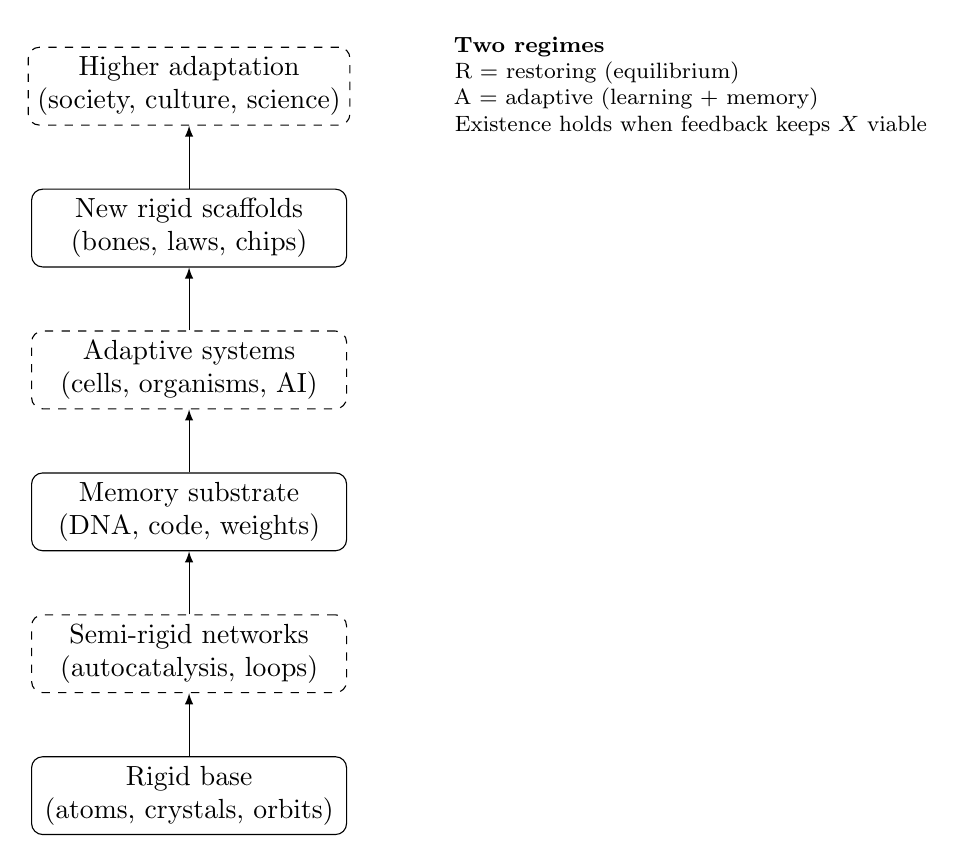
\begin{tikzpicture}[>=latex, node distance=8mm]
\tikzset{
  rigid/.style = {rectangle, rounded corners, draw, align=center, minimum width=40mm, minimum height=7mm},
  adapt/.style = {rectangle, rounded corners, draw, align=center, minimum width=40mm, minimum height=7mm, dashed}
}

% Ladder nodes
\node[rigid] (atoms) {Rigid base\\(atoms, crystals, orbits)};
\node[adapt, above=of atoms] (chem) {Semi-rigid networks\\(autocatalysis, loops)};
\node[rigid, above=of chem] (dna) {Memory substrate\\(DNA, code, weights)};
\node[adapt, above=of dna] (life) {Adaptive systems\\(cells, organisms, AI)};
\node[rigid, above=of life] (infra) {New rigid scaffolds\\(bones, laws, chips)};
\node[adapt, above=of infra] (soc) {Higher adaptation\\(society, culture, science)};

% Edges
\draw[->] (atoms) -- (chem);
\draw[->] (chem)  -- (dna);
\draw[->] (dna)   -- (life);
\draw[->] (life)  -- (infra);
\draw[->] (infra) -- (soc);

% Legend (wrapped to avoid fragile line breaks)
\node[anchor=west] at ([xshift=12mm]soc.east) (legend)
{\begin{minipage}{60mm}\footnotesize
\textbf{Two regimes}\par
R = restoring (equilibrium)\par
A = adaptive (learning + memory)\par
Existence holds when feedback keeps $X$ viable
\end{minipage}};

\end{tikzpicture}

\caption{Alternation of rigid scaffolds (solid) and adaptive layers (dashed). Existence persists when equilibrium feedback (R) and/or adaptive feedback with memory (A) keep the system within its viability region.}
\label{fig:ladder}
\end{figure}

\section{Discussion}
Equation~\eqref{eq:existence} treats existence as a maintained flow.
A pattern endures if either (i) it sits in a self-restoring equilibrium (the $R$ term suffices), or (ii) it learns, stores, and deploys updates that keep it viable (the $A$ term).
In practice, systems intertwine both regimes across time scales: fast signals, medium learning, slow memory.

\section*{References (minimal)}
W.~R. Ashby, \emph{An Introduction to Cybernetics}, Chapman \& Hall, 1956.\\
J.-P. Aubin, \emph{Viability Theory} (2nd ed.), Springer, 2009.\\
M. Eigen, ``Selforganization of matter and the evolution of biological macromolecules,'' \emph{Naturwissenschaften} 58, 465--523 (1971).\\
K. Friston, ``The free-energy principle: a unified brain theory?'' \emph{Nat. Rev. Neurosci.} 11, 127--138 (2010).\\
J.~H. Holland, \emph{Adaptation in Natural and Artificial Systems}, Univ. of Michigan Press, 1975.

\end{document}
